% Created 2022-09-18 Sun 23:06
% Intended LaTeX compiler: pdflatex
\documentclass[11pt,a4paper]{article}
  \usepackage[utf8]{inputenc}
  \usepackage[T1]{fontenc}
  \usepackage{fixltx2e}
  \usepackage{graphicx}
  \usepackage{longtable}
  \usepackage{float}
  \usepackage{wrapfig}
  \usepackage{rotating}
  \usepackage[normalem]{ulem}
  \usepackage{amsmath}
  \usepackage{textcomp}
  \usepackage{marvosym}
  \usepackage{wasysym}
  \usepackage{amssymb}
  \usepackage{hyperref}
  \usepackage{mathpazo}
  \usepackage{color}
  \usepackage{enumerate}
  \definecolor{bg}{rgb}{0.95,0.95,0.95}
  \tolerance=1000
                \usepackage{listings}
\usepackage{xcolor}
\lstset{language=Python,backgroundcolor=\color{black!5}, basicstyle=\footnotesize\ttfamily, columns=fullflexible, breaklines, frame= tb}

  \linespread{1.1}
  \hypersetup{pdfborder=0 0 0}
\author{vijay panchal}
\date{\today}
\title{Timebomb of approximation method in physics}
\hypersetup{
 pdfauthor={vijay panchal},
 pdftitle={Timebomb of approximation method in physics},
 pdfkeywords={},
 pdfsubject={},
 pdfcreator={Emacs 27.1 (Org mode 9.4.6)}, 
 pdflang={English}}
\begin{document}

\maketitle
\tableofcontents



\section{Introduction}
\label{sec:org313d79b}

Approximation method is yet most essential topic in physics. Physicists love to do approximations, like in functional expansion for getting polynomials for their ease or may be specialized idealization in particular topic. Approximation help them to \textbf{doing physics} instead going in to maze of exactness in mathematics. Getting interpretation or more i say knowing system is sometime more important then going for regorious mathematics. For example, famous equation of fluid dynamics \textbf{Navier-Stoke equation} can be imposible to solve but as physicist they know what it is.

Be aware, that approximation is just approximation. We should remember everytime we do that. Sometime we forgot actual system which is far from ideal. We should know that we are on mission to know nature not just building new theories.

Let's dive into one example, what do i imply by consequences of approximation methods. In classical mechanics, we have merely some major theories. In Oscillation theory we studied \textbf{Simple Harmonic Oscillation}, but as we are going to see that simple harmonic oscillation is not exactly that simple. 

\textbf{Write more}

\section{Example of Approximate method}
\label{sec:org8c245ec}

Approximation is very used in almost every in physics. Not, just physics but every field in sciences. We are going to give profound example of understanding advantages and disadvantages of approximation.

\subsection{Defining problem}
\label{sec:org8984ee2}

We learned simple pendulum from early time of physics course. But what if say that simple pendulum is not actually simple in sense that approximation hide most of things away from our eyes to see.

We took physical pendulum. By taking length \(l = 1 m\) string (assuming non expanding) attaching to bob of mass \(m = 0.1 kg\) . String attached to rigid wall as shown in figure. 

\begin{figure}[htbp]
\centering
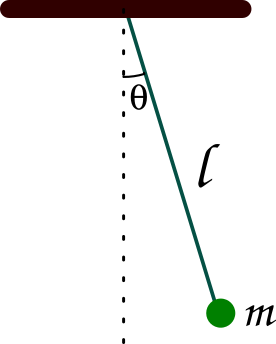
\includegraphics[width=0.3 \textwidth]{./figure1.png}
\caption{\label{fig:org6be9dbd}pendulum with string lenth \(l\) and mass \(m\)}
\end{figure}

For understanding consequences of approximation, we took simulations by solving both equation of motion (approximated and exact). For getting equations of motion we used \textbf{Newtonian formulation} which is quite easy to work with in this type of problems, since we are working with \textbf{non conservative} system. This is our derivation of equation of motion.

First of all, we took horizontal and vertical forces.
\begin{equation}
\label{eq:org09a7556}
   F_{damping}cos(\theta)-Tsin(\theta)=ma_{x}
\end{equation}
\begin{equation}
\label{eq:orge6f8987}
   F_{damping}sin(\theta)+Tsin(\theta)-mg=ma_{y}
\end{equation}

Adding equation \ref{eq:org09a7556} and equation \ref{eq:orge6f8987} with multiplication by \(cos(\theta)\) and \(sin(\theta)\) respectively.

\begin{equation*}
\label{eq:org5a23d30}
F_{damping}sin^{2}(\theta)+F_{damping}cos^{2}(\theta)-mgsin(\theta)=ma_{x}cos(\theta)+ma_{y}sin(\theta)
\end{equation*}

\begin{equation*}
\label{eq:org7279efb}
F_{damping}-mgsin(\theta)=m(asin^{2}(\theta)+acos^{2}(\theta))
\end{equation*}

\begin{equation}
\label{eq:orgaee488c}
F_{damping}-mgsin(\theta)=ma
\end{equation}

From,
\begin{equation*}
\label{eq:orgde960f2}
a = (\ddot{r}-r\dot{\theta}^{2})\hat{r} + (r \ddot{\theta}+2\dot{r}\dot{\theta})\hat{\theta}
\end{equation*}

Where,  \(r=l\) and since \(\dot{l}=0\), \(a=l\ddot{\theta}\). So, equation \ref{eq:orgaee488c} becomes,

\begin{equation*}
\label{eq:org11b111a}
F_{damping}-mgsin(\theta)=ml\ddot{\theta}
\end{equation*}

We are taking damping force to velocity proportional. So, \(F_{damping}=-bl\dot{\theta}\) ( since, \(\dot{l}=0\)). Here, we are assuming that damping is linear. 

\begin{equation*}
\label{eq:org1eb51a8}
-bl\dot{\theta}-mgsin(\theta)=ml\ddot{\theta}
\end{equation*}


Rearranging this equation will give our equation of motion,

\begin{equation}
\label{eq:orga29d2f5}
\ddot{\theta}+\frac{b}{m}\dot{\theta}+\frac{g}{l}sin(\theta)=0
\end{equation}

This is \textbf{exact equation of motion}. Which is \textbf{second order non linear equation}. Finding it's exact solution is massive task. We will use numerical methods to find it's solution. This equation has much more to say than looks. Will learn about this in later.

\subsection{Approximation of equation of motion : Linear differential equation}
\label{sec:org6520315}

Solving \ref{eq:orga29d2f5} is very hard tasks. So, we as physics majors try to make this as friendly as possible. In class, we approximated this as \(\theta \to 0\) as \(sin(\theta) \to \theta\). Consequently, this equation becomes very easy to solve. This becomes,

\begin{equation}
\label{eq:orgc9ebe6e}
\ddot{\theta}+\frac{b}{m}\dot{\theta}+\frac{g}{l}\theta=0
\end{equation}

\begin{equation}
\label{eq:org1446dde}
\ddot{\theta}+\Gamma\dot{\theta}+w_{0}^{2}\theta=0
\end{equation}

Where we took \(\Gamma = \frac{b}{m}\) and \(w_{0}^{2}\).

We can solve this linear equation \ref{eq:org1446dde} by usual methods of linear differential equation. Simply taking \(\theta=e^{\lambda t}\), which gives polynomials of second order.

\begin{equation}
\label{eq:orgd505f63}
\lambda^{2}+\Gamma\lambda+w_{0}^{2}=0
\end{equation}

We can find roots of this quadratic equation.

\begin{equation}
\label{eq:org4a44d7f}
\lambda = \frac{-\Gamma}{2} \pm \frac{\sqrt{\Gamma^{2}-4w_{0}^{2}}}{2}
\end{equation}

\begin{equation}
\label{eq:orgb5d6a37}
\lambda = \frac{-\Gamma}{2} \pm \sqrt{\frac{\Gamma}{2}^{2}-w_{0}^{2}}
\end{equation}

Here we getting three type of roots,

\begin{enumerate}
\item Roots where \(\frac{\Gamma}{2}=w\). this is \textbf{critical damping condition}, where we getting \(\lambda=\frac{-\Gamma}{2}\). Putting \(\lambda\) into our solutions, \(\theta = e^{\frac{-\Gamma}{2}t}\). Which suggest this will only decay with time and never overshoots from equilibrium position. Which is desired in certain condition but not for us.

\item Roots where \(\frac{\Gamma}{2}>w\). this is \textbf{overdamping condition}, where we getting \(\lambda=\frac{-\Gamma}{2}\pm\sqrt{\frac{\Gamma}{2}^{2}-w_{0}^{2}}\). So from here we get \(\theta = e^{\frac{-\Gamma}{2}t}e^{\pm\sqrt{\frac{\Gamma}{2}^{2}-w_{0}^{2}}t}\). This also have exponential term in it which will only decay with time and never overshoots from equilibrium position.

\item Roots where \(\frac{\Gamma}{2}<w\). this is \textbf{underdamping condition}, here  \(\lambda=\frac{-\Gamma}{2}\pm i\sqrt{w_{0}^{2}-\frac{\Gamma}{2}^{2}}\). \(\theta = e^{\frac{-\Gamma}{2}t}e^{\pm i \sqrt{w_{0}^{2}-\frac{\Gamma}{2}^{2}}t}\). This has complex term, which implicitly suggest that it'll overshoot and oscillate. This our topic of interest for this project.
\end{enumerate}



\textbf{Solve linear equation}

\subsection{Simulations}
\label{sec:org51ee064}
\subsubsection{Understand Runge-Kutta method}
\label{sec:org724955b}

\subsubsection{Animations}
\label{sec:org129aeed}




I done animation with python's pygame library which is acurate in time. This library make sures that our system follows as real life as possible.

\begin{lstlisting}[language=Python]
    def bob1(window,x,y):
        image = pygame.image.load("bitmap2.png")
        window.blit(image, (x,y))

    def bob2(window,x,y):
        image = pygame.image.load("bitmap.png")
        window.blit(image, (x,y))

    def surface(window,x,y):
        image = pygame.image.load("drawings.png")
        window.blit(image, (x, y))
    
    def position(l,theta):
        return origin_x-10+l*cos((1.5*pi)-theta),origin_y-10-l*sin((1.5*pi)-theta)
    
    def mainloop(window,fps):
        global t
        run = True
        clock = pygame.time.Clock()
        c = 0
        while run:
            for event in pygame.event.get():
                if event.type== pygame.QUIT:
                    run= False
                    break
            clock.tick(fps)

            x,y = position(l,exact[c])
            x2,y2 = position(l,appro[c])
            if c==len(exact):
                break
            window.fill("#ffffff")
            surface(window,175,origin_y-25)
            pygame.draw.aaline(window,color="#5BDEC1",start_pos=(origin_x,origin_y),end_pos=(x+radius,y+radius))
            pygame.draw.aaline(window,color="#5BDEC1",start_pos=(origin_x,origin_y),end_pos=(x2+10,y2+10))
            bob1(window,x,y)
            bob2(window,x2,y2)
            pygame.display.update()
            c+=1
        pygame.quit()

    if __name__ == "__main__":
        pygame.init()
        window = pygame.display.set_mode((width,height))
        exact = nonlinear(5,30)
        appro = linear(5,30)
        t = time.perf_counter()
        mainloop(window, 30)
\end{lstlisting}

\section{What is meaning of all this ?}
\label{sec:org0b3d3c5}
\end{document}